%%%%%%%%%%%%%%%%%%%%%%%%%%%%%%%%%%%%%%%%%
% Short Sectioned Assignment
% LaTeX Template
% Version 1.0 (5/5/12)
%
% This template has been downloaded from:
% http://www.LaTeXTemplates.com
%
% Original author:
% Frits Wenneker (http://www.howtotex.com)
%
% License:
% CC BY-NC-SA 3.0 (http://creativecommons.org/licenses/by-nc-sa/3.0/)
%
%%%%%%%%%%%%%%%%%%%%%%%%%%%%%%%%%%%%%%%%%

%----------------------------------------------------------------------------------------
%	PACKAGES AND OTHER DOCUMENT CONFIGURATIONS
%----------------------------------------------------------------------------------------

\documentclass[paper=a4, fontsize=14pt, xcolor=dvipsnames]{scrartcl} % A4 paper and 11pt font size

\usepackage[T1]{fontenc} % Use 8-bit encoding that has 256 glyphs
\usepackage{fourier} % Use the Adobe Utopia font for the document - comment this line to return to the LaTeX default
\usepackage{amsmath,amsfonts,amsthm} % Math packages
\usepackage{natbib}
\usepackage{pgfplots}

% Bibliographie auf deutsch
%\usepackage{harvard}
%\renewcommand{\harvardand}{und} 

\usepackage{xcolor}
\usepackage[utf8]{inputenc} 
\usepackage[ngerman]{babel}

\usepackage{latexsym}
\usepackage{textcomp}
\usepackage[T1]{fontenc}
\usepackage{bm}% bold math
\usepackage{hyperref}
\usepackage{graphicx}
\usepackage{epsfig}
\usepackage{framed,color}
\usepackage[usenames,dvipsnames]{pstricks}
\usepackage{epsfig}
\usepackage{tikz}
\usepackage{lipsum} % Used for inserting dummy 'Lorem ipsum' text into the template
\usepackage{sectsty} % Allows customizing section commands
\allsectionsfont{\centering \normalfont\scshape} % Make all sections centered, the default font and small caps

\usepackage{fancyhdr} % Custom headers and footers
\pagestyle{plain} % Makes all pages in the document conform to the custom headers and footers
\fancyhead{} % No page header - if you want one, create it in the same way as the footers below
\fancyfoot[L]{} % Empty left footer
\fancyfoot[C]{} % Empty center footer
\fancyfoot[R]{\thepage} % Page numbering for right footer
%\renewcommand{\headrulewidth}{0pt} % Remove header underlines
%\renewcommand{\footrulewidth}{0pt} % Remove footer underlines
\setlength{\headheight}{13.6pt} % Customize the height of the header
\usepackage{eso-pic}
\numberwithin{equation}{section} % Number equations within sections (i.e. 1.1, 1.2, 2.1, 2.2 instead of 1, 2, 3, 4)
\numberwithin{figure}{section} % Number figures within sections (i.e. 1.1, 1.2, 2.1, 2.2 instead of 1, 2, 3, 4)
\numberwithin{table}{section} % Number tables within sections (i.e. 1.1, 1.2, 2.1, 2.2 instead of 1, 2, 3, 4)

\setlength\parindent{0pt} % Removes all indentation from paragraphs - comment this line for an assignment with lots of text

%----------------------------------------------------------------------------------------
%	TITLE SECTION
%----------------------------------------------------------------------------------------

\newcommand{\horrule}[1]{\rule{\linewidth}{#1}} % Create horizontal rule command with 1 argument of height

\title{ 
\normalfont \normalsize 
\textsc{Albert-Ludwigs-Universität Freiburg} \\ [25pt] % Your university, school and/or department name(s)
\horrule{0.5pt} \\[0.4cm] % Thin top horizontal rule
\huge Rastertunnelmikroskop \\ % The assignment title
\horrule{2pt} \\[0.5cm] % Thick bottom horizontal rule
}

\author{Friedrich Schüßler und Volker Karle} % Your name

\date{\normalsize\today} % Today's date or a custom date

\begin{document}
\maketitle

\tableofcontents
\thispagestyle{empty}
\newpage
\setcounter{page}{1}


%----------------------------------------------------------------------------------------
%	PROBLEM 1
%----------------------------------------------------------------------------------------

\section{Einführung}
\section{Einführung in die Rastertunnelmikroskopie}
In der Rastertunnelmikroskopie (engl. \textit{scanning tunneling
microscope}, \textbf{STM}) wird die Oberfläche von Festkörpern auf atomarer 
Größenskala untersucht. Dabei wird der quantenmechanische Tunneleffekt 
ausgenutzt, der einen minimalen Stromfluss dort erlaubt, wo klassisch 
die Potentialbarriere zu hoch wäre. Eine Spitze, die im Idealfall mit 
einem Atom endet, fährt die Oberfläche in einem festen Raster am, während 
ein Computer Stromfluss im nA-Bereich und die Verschiebung misst. 
Die Wahrscheinlichkeit, dass ein Elektron durch die Potentialbarriere 
zwischen Oberfläche und Spitze ”tunnelt”, hängt stark von dem Abstand 
dazwischen ab – daher kann der Tunnelstrom als Messgröße für diesen 
Abstand benutzt werden. Mit Hilfe des entsprechenden theoretischen 
Zusammenhanges und Modellen aus der Festkörperphysik können so Bilder 
von der Geometrie der Oberfläche erstellt werden und beispielsweise 
Parameter wie die Gitterkonstante berechnet werden. Gängige Auflösungen liegen
bei 0.1 nm in der Ebene sowie 0.01 nm in der Tiefe. Untersucht werden in 
diesem Versuch die Oberflächen von Graphit, einer mit Gold beschichteten 
Struktur und des Halbleiters $\mathrm{MoS_2}$. 


\subsection{Historischer Abriss}
Die ursprüngliche Idee der Erfinder des RTMs 
war es nicht, ein Mikroskop zu konstruieren,
sondern Spektroskopie in einer Größenordnung von 
100 \r{A} durchzuführen \cite{binnig1987scanning}.
Mit der ersten experimentellen Realisation \cite{thompson1976thermal}
des Tunnelns mit einer positionierbaren Spitze tauchte das 
das Konzept des Tunnelns in der 
Festkörperphysik auf, als versucht wurde, durch Vakuum bzw. durch
eine Vakuumbarriere zu tunneln \cite{binnig1982tunneling}. 
Erst dann wurde festgestellt, das mit dieser Methode nicht nur
Spektroskopie, sondern eine neue Art des Mikroskops entwickelt werden
konnte.
Diese
waren zunächst aufgrund der Vibrationen nicht erfolgreich. Nun sind
die Vorteile des Vakuumtunnelns aber evident: 
Zum einen handelt es sich um die konzeptuell am einfachsten
herzustellende Barriere, zum anderen ist ein freier Zugang 
der Elektroden für die Untersuchung anderer
physikalischer und chemischer Prozesse möglich.
Die Fragen, die sich in diesem Zusammenhang
ergaben und gelöst bzw. beantwortet werden mussten, waren:

\begin{enumerate}
\item Wie können die mechanischen Vibrationen, die die Spitze
erschüttern und sich gegenseitig aufschaukeln, unterdrückt bzw.
verringert werden?
\item Wie stark sind die (Anziehungs-)kräfte zwischen der Spitze
und der Probe? Wie sollte die Form der Spitze aussehen und wie
ist es möglich eine solche Form auf dieser Skala herzustellen?
\end{enumerate}

1981 führten die Autoren G.Binnig, H.Rohrer,
Ch.Gerber und E.Weibel in Zürich zum ersten Mal ein erfolgreiches
Tunnelexperiment \cite{binnig1982tunneling} 
mit einem justierbarem Vakuum Spalt durch. 
Ziel war hierbei, das Phänomen des Tunnelns so zu erforschen,
um es in der Spektroskopie und andere Methoden einsetzen zu können. 
Offensichtlich war der schwierige Teil der, die Vibrationen,
die vergangene Experimente fehlschlugen ließen, hinreichend zu
unterdrücken, um somit das eigentliche Signal noch identifizieren zu
können. Dies wurde in dem erwähnten Experiment durch eine 
Dämpfung des Tunnelbauteils erreicht, und zwar durch einen Schutz
von akkustischen Rauschen durch eine das Mikroskop umgebende 
Suspension innerhalb einer Vakuumkammer. 
Mithilfe von Leviation durch Supraleiter-induzierte Magneten sowie
der Steuerung mit Piezoelementen erfolgt das Abrastern einer
Probe. \\ Der Trick liegt darin,
die charakteristischen Frequenzen so zu wählen, dass die 
Eigenfrequenzen des Materials für Vibrationen weit darüber liegen.
Dies ist möglich, indem die Größe des Bauteils sehr klein
skaliert wird, somit können sich keine Vibrationen ausbilden.
Für die erste Realisation eines RTMs  
wurde Gerd Binnig und Heinrich Rohrer 1986 der \textbf{Nobelpreis
für Physik} verliehen. 
Die Frage nach der Form der Spitze ist komplizierter, da es 
nicht unbedingt möglich ist, die Spitze als Sphere mit einer
bestimmten Krümmung und Radius zu beschreiben, da die Rauheit der
Spitze die Existenz vieler kleiner Spitzen implizieren. Diese
sogenannten \textit{Minispitzen} reagieren sehr sensitiv auf die anliegende
Tunnelstromstärke; die jeweils näheste bildet dann die Verbindung
zur Probe (siehe Abbildung~\ref{fig:multitip}).\\ 
\begin{figure}
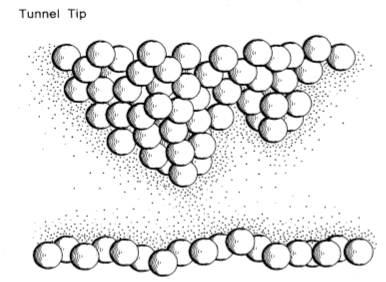
\includegraphics[width=7cm]{pics/multitip}
\caption{ Schematische Abbildung aus \cite{binnig1987scanning}
auf der der die strukturelle Aufbau der Spitzen und der Probe 
zu sehen ist.} 
 \label{fig:multitip}
\end{figure}
Die erste Anwendung, welche die RTMs bekannt
machte, war die Oberflächenrekonstruktion von Silizium(111)  
\cite{binnig19837} (siehe Abbildung~\ref{fig:silicium}).
Dabei handelte es sich um ein offenes Problem in der
Festkörperphysik. Wie sich später durch die experimentelle
Aufarbeitung zeigte, waren die theoretischen Vorhersagen nicht 
korrekt und mussten korrigiert werden, gerade auch deswegen
erlangte die Rastertunnelmikroskopie ab 1985 große Bekannheit.
\begin{figure}
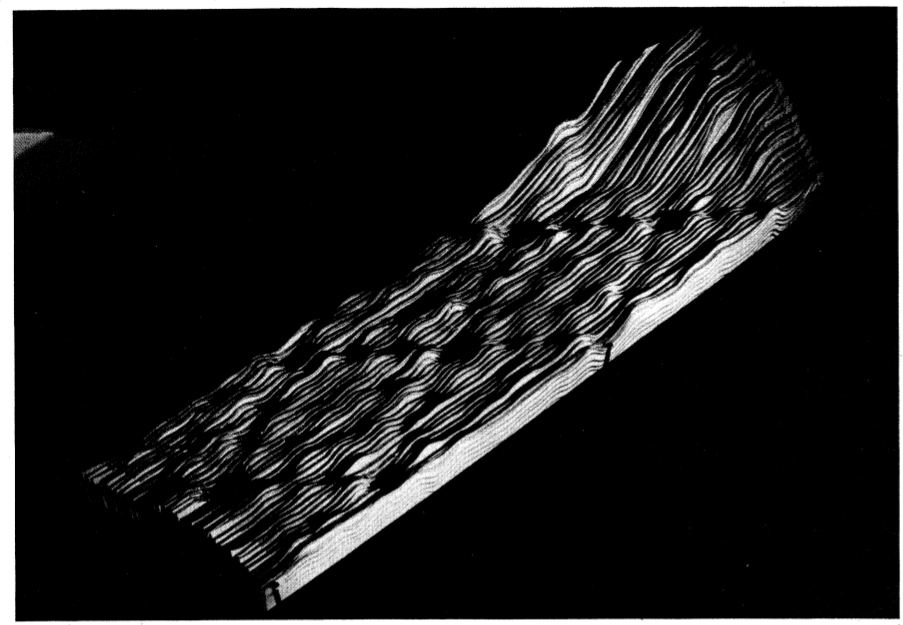
\includegraphics[width=7cm]{pics/silicium}
\caption{Erste Anwendung des Rastertunnelmikroskops 
\cite{binnig19837}: 
Oberflächenrekonstruktion von Silizium(111) (siehe Millersche
Indizes im Theorieteil), welches eine komplexe (7x7) 
Überstrukturzelle besitzt}
 \label{fig:silicium}
\end{figure}

Auf ihr baut die gesamte Rastersondenmikroskopie auf, welche
in einigen Spielarten in der Zeit danach weiterentwickelt wurde.
So war ist mit dem \textit{Rasterkraftmikroskop}
und dem \textit{optische Rasternahfeldmikroskop} möglich, sogar
nichtleitende Proben zu untersuchen, da das Abrastern nicht auf
einen geschlossenen Stromkreis basiert, sondern auf Kräften 
atomarer Ebene (Coulomb, Pauliprinzip). Somit bilden sie die Basis
für viele Anwendungen in der Chemie und Biologie.\\
1993 gelang es M.F. Crommie, C.P.Lutz und
D.M Eigler \cite{crommie1993imaging} dann
ein \textit{Quantengehege} aufzubauen
(engl. \textit{Quantum Corral}). Somit konnten mithilfe
des RTMs sogar Interferenzphänomene von Atomen
sichtbar gemacht werden (siehe Abbildung~\ref{fig:quantum_corral}. 

\begin{figure}
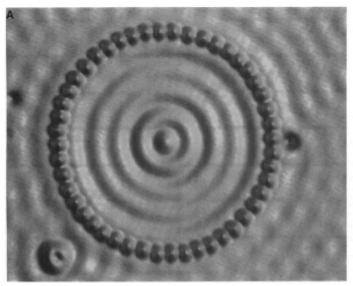
\includegraphics[width=7cm]{pics/quantum_corral}
\caption{Die Abbildung zeigt die 
    Visualisierung des Quantumgeheges, welches 1993 von 
    Crommie, Lutz und Eigler mithilfe des RTMs 
    konstruiert werden konnte \cite{crommie1993imaging}. 
    Speziell in dieser Abbildung ist eine 48-Eisen-atomige 
Ring konstruktion zu sehen, welche auf Kupfer(111) aufgebaut wurde.
Der Durchschnittsdurchmesser des Rings beträgt 142.6\r{A}.}
 \label{fig:quantum_corral}
\end{figure}


\section{Theorie des Quantentunnelns}
\textit{Quantentunneln}, oder kurz \textit{Tunneln} 
bezeichnet das quantenmechanische Phänomen, wenn 
die Durchtrittswahrscheinlichkeit eines Teilchens
durch eine Potenzialbarriere nicht null ist, selbst wenn die Energie
des Teilchens geringer ist als das Potenzial selbst ($E < V$), was
in der klassischen Mechanik nicht möglich wäre. Dies
spielt eine wichtige Rolle bei
vielen Phänomenen in Natur und Technik,
beispielsweise bei der Kernfusion der Sonne, bei der Diode und
daher auch beim Transistor und somit bei der Funktionionsweise
eines Computers an sich, aber auch beim Quantencomputer oder
eben in unserem Fall beim RTM. Das Phänomen des Quantentunnelns
wurde Anfang des 20ten Jahrhunderts mit der Entdeckung der 
Quantenmechanik postuliert und Mitte des Jahrhunderts bestätigt.
\subsection{Mathematische Herleitung von Quantentunneln}
In den folgenden Ausführungen werden Kenntnisse der Quantenmechanik
vorrausgesetzt. Betrachten wir zunächst die Zeitunabhängige
Schrödingergleichung für ein Teilchen in einer Dimension:
\begin{align}
\left [ \frac{-\hbar^2}{2m}\partial_x^2 + V(x) \right ]\psi(x) = E\psi(x) \\ 
\Leftrightarrow \left [ \frac{-\hbar^2}{2m}\partial_x^2 \right ]\psi(x) = \left [E-V(x) \right ]\psi(x) 
\end{align}
Im Spezialfall wenn $V(x)$ konstant ist, können wir die Gleichung
sofort mit planaren Wellen lösen:
\begin{align}
    k^2 = \frac{2m}{\hbar^2}(V-E)\\
    \psi(x) \sim \exp(kx) 
\end{align}
Wenn $V(x)$ nicht konstant ist, können wir mithilfe der WKB-Methode 
\cite{froman1970transmission}
immerhin noch den Transmissionskoeffizienten berechnen, sofern
das Potenzial zwischen zwei Rändern $x_1$ und $x_2$ eingespannt ist 
und ausserhalb davon null wird. Dazu setzen wir für die 
Wellenfunktion $\psi(x)=\exp(\phi(x))$ an, 
mit einer komplexen Funktion $\phi(x)$. 


\section{Theoretische Grundlagen}

\newcommand{\VG}{V_{\mathbf{G}}}
\newcommand{\G}{\mathbf{G}}
\newcommand{\g}{\mathbf{g}}
\newcommand{\R}{\mathbf{r}}
\newcommand{\K}{\mathbf{k}}
\newcommand{\A}{\mathbf{a}}
\newcommand{\ex}{\mathbf{e}^}
\subsection{Theorie des Quantentunnelns}
\textit{Quantentunneln}, oder kurz \textit{Tunneln} 
bezeichnet das quantenmechanische Phänomen, wenn 
die Durchtrittswahrscheinlichkeit eines Teilchens
durch eine Potenzialbarriere nicht null ist, selbst wenn die Energie
des Teilchens geringer ist als das Potenzial selbst ($E < V$), was
in der klassischen Mechanik nicht möglich wäre. Dies
spielt eine wichtige Rolle bei
vielen Phänomenen in Natur und Technik,
beispielsweise bei der Kernfusion der Sonne, bei der Diode und
daher auch beim Transistor und somit bei der Funktionionsweise
eines Computers an sich, aber auch beim Quantencomputer oder
eben in unserem Fall beim RTM. Das Phänomen des Quantentunnelns
wurde Anfang des 20ten Jahrhunderts mit der Entdeckung der 
Quantenmechanik postuliert und Mitte des Jahrhunderts bestätigt.
\subsection{Mathematische Herleitung von Quantentunneln}
In den folgenden Ausführungen werden Kenntnisse der Quantenmechanik
vorrausgesetzt. Betrachten wir zunächst die Zeitunabhängige
Schrödingergleichung für ein Teilchen in einer Dimension:
\begin{align}
\left [ \frac{-\hbar^2}{2m}\partial_x^2 + V(x) \right ]\psi(x) = E\psi(x) \\ 
\Leftrightarrow \left [ \frac{-\hbar^2}{2m}\partial_x^2 \right ]\psi(x) = \left [E-V(x) \right ]\psi(x) 
\end{align}
Im Spezialfall wenn $V(x)$ konstant ist, können wir die Gleichung
sofort mit planaren Wellen lösen:
\begin{align}
    k^2 = \frac{2m}{\hbar^2}(V-E)\\
    \psi(x) \sim \exp(ikx) 
\end{align}
\subsubsection{Rechteckspotenzial}
Nehmen wir nun an, das Potenzial ist gegeben durch:
\begin{equation}
    V(x) = V_0 \left [ \Theta(x) - \Theta(x-a) \right ] 
\end{equation}
Wobei $\Theta(x)$ die Heavisidefunktion ist und $V_0 > E$.
Die Barriere teilt den Raum nun in drei Teile, $x<0$, $0\leqslant x\leqslant a$ und $a<x$.
In jedem dieser Teile ist das Potenzial konstant, somit können wir für jeden Teil eine
obere Lösung ansetzen \cite{wolfgang2010experimentalphysik},
\cite{landau1991quantenmechanik}:
\begin{align}
    \psi_I(x)    &= A_r \exp(ik_0x) + A_l  \exp(-ik_0x) \mbox{ for } x<0\\
    \psi_{II}(x) &= B_r \exp(ik_1x) + B_l  \exp(-ik_1x) \mbox{ for } 0 \leqslant x \leqslant a\\
    \psi_{III}(x)&= C_r \exp(ik_0x) + C_l  \exp(-ik_0x) \mbox{ for } x>0
\end{align}
Für $E>V_0$ gilt nun:
\begin{align}
    k_0 &= \frac{\sqrt{2mE}}{\hbar}\\
    k_1 &= \frac{\sqrt{2m(E-V_0)}}{\hbar}
\end{align}
Die Koeffizienten A,B und C lassen sich nun mit den Randbedingungen
für die Stetigkeit lösen:
\begin{align}
    \psi_I(0)&\overset{!}{=} \psi_{II}(0)\\
    (\partial_x\psi_I)(0)&\overset{!}{=} (\partial_x\psi_{II})(0)\\
    \psi_{II}(a)&\overset{!}{=} \psi_{III}(a)\\
    (\partial_x\psi_{II})(a)&\overset{!}{=} (\partial_x\psi_{III})(a)
\end{align}
Dies ergibt nach einsetzen der Lösungen für die Wellenfunktionen:
\begin{align}
  A_r + A_l &= B_r + B_l \\
  ik_0(A_r-A_l) &= ik_1(B_r-B_l)\\
  B_r\exp(iak_1)+B_l\exp(-iak_1)&=C_r \exp(iak_0)+C_l\exp(-iak_0)\\
  ik_1(B_r\exp(iak_1) - B_l\exp(-iak_1))&=ik_0(C_r\exp(iak_0)-C_l\exp(-iak_0))
\end{align}
Dies sind 6 freie Parameter für 4 Gleichungen, also können wir zwei 
Paramter festsetzen. Wir setzen $A_r =1$ (Skalierung nach der einlaufenden
Welle) und $C_l = 0$, das bedeutet, dass keine Welle von rechts dazukommt,
sondern alles von der einlaufenden Welle $A_r$ abhängt. Des weiteren
benennen wir $A_l=r$ für Reflexion, und $C_r=t$ für Transmission. Nun
lassen sich die Gleichungen nach diesen Koeffizienten auflösen:
\begin{align}
    t &= \frac{4k_0k_1\exp(-ia(k_0-k_1))}{(k_0+k_1)^2 - \exp(2iak_1)(k_0-k_1)^2}\\
    r &= \frac{(k_0^2 - k_1^2)\sin(ak_1)}{2ik_0k_1\cos(ak_1)+(k_0^2+k_1^2)\sin(ak_1)}
\end{align}
Nun lässt sich mit diesen Ausdrücken die Übergangswahrscheinlichkeit durch die 
Barriere berechnen:
\begin{align}
    T = \left | t \right |^2 = \frac{1}{1 + \frac{V_0^2 \sinh^2(k_1a)}{4E(V_0-E)}}
    \label{eq:T1}
\end{align}
Wenn das Potenzial kleiner ist als die Energie, läuft die Rechung analog
(wobei $k_1 = \frac{\sqrt{2m(V_0-E)}}{\hbar}$) und wir erhalten:
\begin{align}
    T = \left | t \right |^2 = \frac{1}{1 - \frac{V_0^2 \sin^2(k_1a)}{4E(V_0-E)}}
    \label{eq:T2}
\end{align}

\begin{figure}

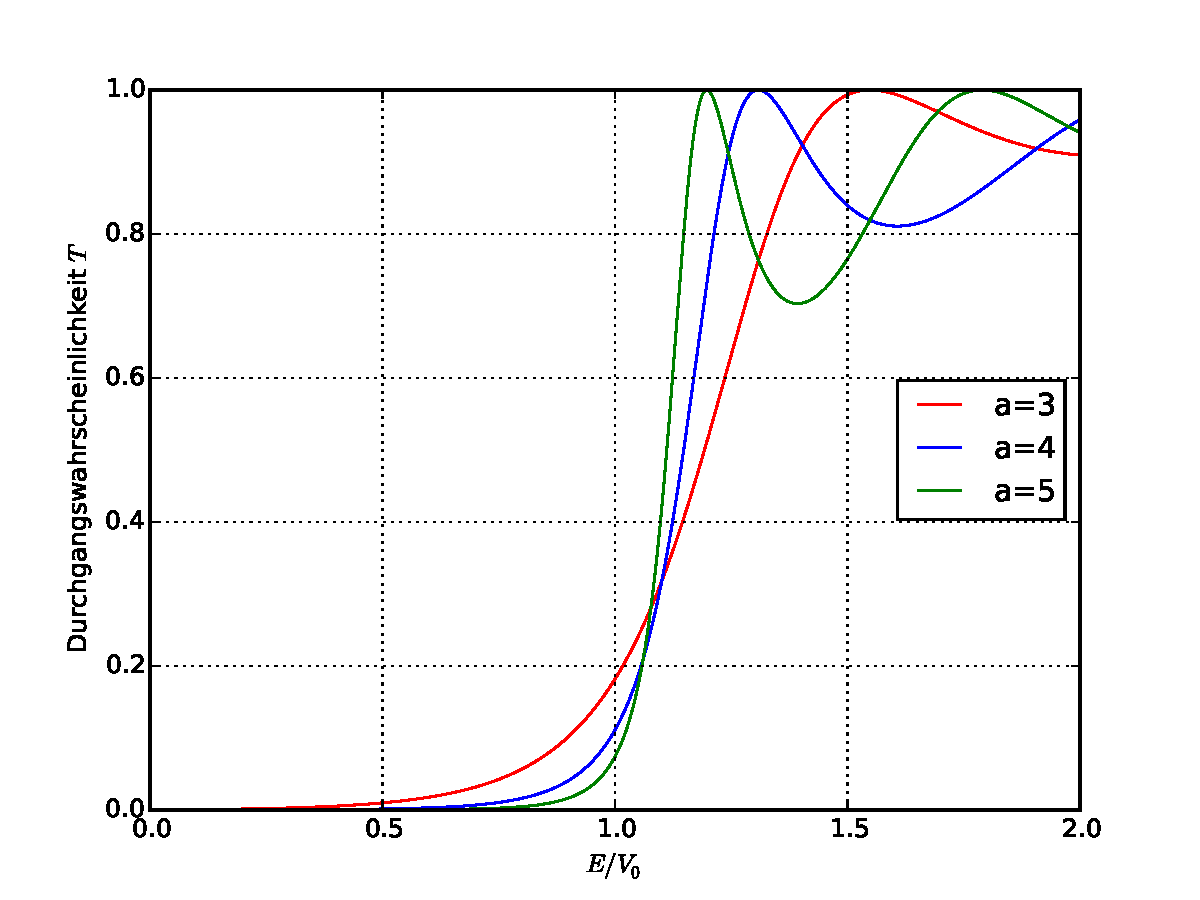
\includegraphics[width=14cm]{pics/tunnel1}
\caption{Transmissionswahrscheinlichkeit nach Gleichung~\ref{eq:T1} und Gleichung~\ref{eq:T2}
bei verschiedenen Breiten des Potenzials $a$ (obdA wurde hier $\hbar=1$ und $m=1$ gewählt).
Hier wird deutlich ersichtlich, inwiefern sich der Quantenmechanische Fall vom klassischen
Fall unterscheidet, so ist die Wahrscheinlichkeit für Energien kleiner als das Potenzial ungleich
null und auch bei höheren Energien nicht konstant eins.} 

 \label{fig:tunnel1}
\end{figure}

\subsubsection{Tunneleffekt beim Rastertunnelmikroskop}
Im eben besprochenen Fall der eindimensionalen Potenzialwand zeichnet sich schon das
assymptotische Verhalten für $a\gg1$ ab:
\begin{equation}
    T = \left | t \right |^2 \overset{\kappa a \gg 1}{\rightarrow} (\frac{4k_1k_0}{k_1^2+k_0^2})^2 
    \exp(-2k_1a)
\end{equation}
Dies ist unter den vielen Bedingungen nur eine grobe Näherung für die Tunnelmikroskopie, doch
diese Näherung stimmt gut mit einem detaillierteren Ansatz überein.
Nehmen wir nun an, dass eine Spitze, bestehend aus einem Atom, sich der zu mikroskopierenden
Oberfläche nähert. Nehmen wir nun weiter an, dass unter Anliegen einer Spannung ein Tunnelstrom
zwischen der Spitze und der Oberfläche der Probe fliesst, wie lässt sich nun der Tunnelstrom
approximieren? Der Tunneleffekt führt dazu, dass die näherungsweise durch das Vakuum 
dargestellte Potenzialwand der Länge $d$ durch die Elektronen überwunden wird (siehe
Abbildung~\ref{fig:tersoff_hamann}). Die Elektronendichte an der Spitze kann nun näherungsweise
mit einer S-Wellenfunktion angegeben werden\cite{staatsexamen}. 
Nun wird die lokale Oberflächendichte $\rho(r)$ an
der Fermioberfläche (siehe die theoretische Einführung
im nächsten Kapitel) durch die Spitze gemessen. Der Radius $R$ des wahrscheinlichsten Aufenthalts
des Elektrons (siehe Abbildung~\ref{fig:tersoff_hamann}) und die Position $r_0$ der Spitze 
bestimmten nun, welcher Tunnelstrom fliessen kann.
Für den Tunnelstrom erhält man:
\begin{equation}
    I \sim U \exp(-2k(R+d)) \rho(r_0,E_f)
\end{equation}
Für die Auflösung des Tunnelmikroskops erhalten wir umgehend
\begin{equation}
    L \sim \sqrt{R+d} 
\end{equation}
Im folgenden wollen wir darauf eingehen, auf welche Weise die Festkörpereigenschaften
durch quantenmechanische Modelle dargestellt werden können. 
\begin{figure}
    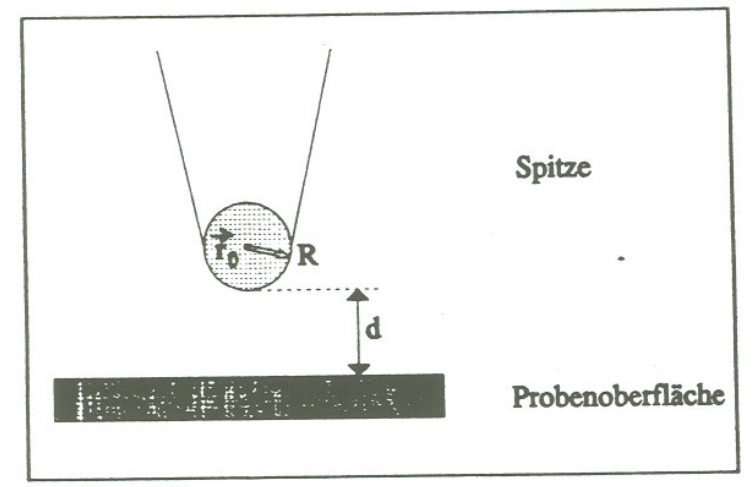
\includegraphics[width=14cm]{pics/tersoff_hamann}
    \caption{Das sogennante Tersoff-Hamann Standardmodell, welches in
        der Modellierung für die Rastertunnelmikroskopie in der Näherung
        für eine räumlich ausgedehnte Tunnelspitze herangezogen wird.
        Abbildung aus \cite{staatsexamen}.}
\label{fig:tersoff_hamann}
\end{figure}

\subsection{Charakterisierung von Kristallgittern}
Vor der Beschreibung der Oberflächen von Kristallen wenden wir uns dem darunter liegenden 
Gitter zu, das die Basis für die Oberfläche darstellt. Die charakteristischen Größen 
sind auch für die Oberflächen wichtig. Die Untersuchung der Kristallgitter findet vor 
allem durch Beugungsexperimente statt, da diese die periodische Struktur am besten 
ausnutzen und so zu höherer Genauigkeit kommen als direkte Abbildung der Oberflächen. 

Fundamental für die Beschreibung der Phänomene der Festkörperphysik ist der reziproke 
oder $\K$-Raum. Er ist aus den $\K$-Vektoren ebener Wellen aufgebaut, die mit 
$\ex{i \K \cdot \R}$ beschrieben werden. Sind nun 
die Gittervektoren eines Kristalles im Ortsraum mit $\A_1,\ \A_2,\ \A_3$ gekennzeichnet, 
so gilt für die reziproken Gittervektoren $\g_1,\ \g_2,\ \g_3$:
\begin{eqnarray}
    \g_1 = 2 \pi \frac{\A_2 \times \A_3 }
        {\A_1\cdot (\A_2 \times \A_3)} \qquad \mathrm{und \ zyklisch} \\
    \mathbf{g_i} \cdot \mathbf{a_j} = 2 \pi \delta_{ij}
\end{eqnarray}
Die periodische Struktur des Kristalles bleibt also im reziproken Raum erhalten.
Ein beliebiger Vektor $\G$ des reziproken Gitters lässt sich als ganzzahlige Linearkombination 
der Basisvektoren darstellen.
\begin{equation}
    \mathbf{G} = h \mathbf{g_1} + k \mathbf{g_2} + l \mathbf{g_3} \mbox{ mit }h,k,l \in \mathbb{Z}
\end{equation}
Für einen Vektor $\R$, der auf dem Gitter im Ortsraum liegt, gilt dann also:
\begin{eqnarray}
    \mathbf{r} &=& n_1 \mathbf{a_1} + n_2 \mathbf{a_2} + n_3 \mathbf{a_3} \\
    \mathbf{G} \cdot \mathbf{r}&=& 2 \pi m  \\
    n_1, \, n_2, \, n_3, \, m &\in& \mathbb{Z}
\end{eqnarray}

Schließlich lässt sich jede Funktion, die im Ortsraum periodisch ist, als 
Fourierreihe im reziproken Raum darstellen:
\begin{equation}
    f(\R) = \sum_{\G} F_{\G} \ex{i \G \cdot \R}
\end{equation}

Bei der Bezeichnung der Netzebenen werden die sogenannten Millerschen Indizes benutzt. 
Spannt man mit drei nicht auf einer Geraden liegenden Gitterpunkten eine Ebene, so ist 
diese durch 
drei ganze Zahlen $m, n, o$ gekennzeichnet. Aus diesen erhält man ein teilerfremdes 
Triplet $(h, k, l)$, indem man die reziproken Werte $h' = 1/m, k' = 1/n, l' = 1/o$ mit 
einer ganzen Zahl $p$ multipliziert. Der reziproke 
Gittervektor $\G$ steht nun senkrecht auf dem mit $(h, k, l)$ beschriebenen Gitter.
\cite{ibach2009festkorperphysik}


\subsection{Blochtheorie und Bändermodell}

Für die Rastertunnelmikroskopie ist die räumliche Verteilung der Elektronen an 
der Oberfläche von zentraler Bedeutung. Die Blochtheorie macht Aussagen über 
die Aufenthaltswahrscheinlichkeiten von Elektronen in periodischen 
Gittern und liefert ein Modell zur Erklärung des Bändermodells. 
Für ein Elektron mit Wellenfunktion $\psi$ gilt bei Vernachlässigung der 
Elektron-Elektron-Wechselwirkung in der nichtrelativistischen Näherung die 
Schrödingergleichung 
\begin{equation}
    \hat H \psi(\R) = \Big[ - \frac{\hbar^2}{2m} \Delta + V(\R) \Big] \psi(\R) = E \psi(\R)
\end{equation}
mit periodischem Potential
\begin{equation}
    V(\R) = V(\mathbf{r + r_n}); 
\qquad \mathbf{r_n} = n_1 \mathbf{a_1} + n_2 \mathbf{a_2} + n_3 \mathbf{a_3} 
\end{equation}
wobei $\mathbf{a_i}$ Gittervektoren des Ortsraumes sind. Auf Grund der Periodizität lässt 
sich das Potential in eine Fourierreihe zerlegen:
\begin{eqnarray}
    V(\R) &= &\sum_\G \VG \mathrm{e}^{i\G \cdot \R} \\
    \mathrm{mit \ Fourierkomponente \quad}  \VG &= &\frac{1}{L} \int \mathrm{e}^{i\G \cdot \R} 
    V(\R) \mathrm{d}\R  \nonumber \\
    \mathrm{und \ reziprokem \ Gittervektor \quad} \G &= &h\mathbf{g_1} + k\mathbf{g_2} +l\mathbf{g_3}; 
    \quad h, \ l, \ k, \ \in \mathbb{Z}. \nonumber
\end{eqnarray}

Der Ansatz für die Lösung ist eine Linearkombination ebener Wellen
$ \psi(\R) = \sum_\K C_\K \mathrm{e}^{i\K \cdot \R}, $
für die nach Einsetzen in die Schrödingergleichung gelten muss:
\begin{equation}
    \sum_\K \mathrm{e}^{i\K \cdot \R} 
    \Big[ \Big( \frac{\hbar^2 k^2}{2m} - E\Big) C_\K + \sum_\G \VG C_{\K - \G}\Big] 
    = 0
\end{equation}
Aus der Unabhängigkeit von $\R$ folgt dann
\begin{equation}
    \Big( \frac{\hbar^2 k^2}{2m} - E\Big) C_\K + \sum_\G \VG C_{\K - \G}= 0
\end{equation}

Zu jeden $\K$ Wert ergeben sich also $N$ Gleichungen, die die Koeffizienten
$C_\K$ jeweils mit $C_{\K - \G'}$, $C_{\K - \G''}$,\ldots  koppeln, wobei $N$ die Anzahl 
der Elementarzellen im Gitter ist. Daher lassen sich die Wellenfunktionen 
mit Energie $E_\K$ also Superposition ebener Wellen schreiben, deren $\K$ Werte 
alle auf dem reziproken Gitter liegen: 

\begin{eqnarray}
    \psi_\K(\R)&=& \sum_\G C_{\K - \G} \mathrm{e}^{i(\K - \G) \cdot \R} \nonumber \\
            &=& \sum_\G C_{\K - \G} \mathrm{e}^{i \G \cdot \R}  \mathrm{e}^{i\K \cdot \R} \nonumber \\
            &=& u_\K(\R) \cdot \mathrm{e}^{-i\K \cdot \R} 
\end{eqnarray}

Diese Wellenfunktionen werden Bloch-Wellen genannt. Das Bloch-Theorem sagt aus, 
dass für das Einelektronenproblem im periodischen Potential eben diese Bloch-Wellen 
Energie-Eigenfunktionen mit Eigenwerten $E_\K$ mit $\K = \frac{2 \pi}{L} (n_x, n_y, n_z)$ und
\begin{equation}
    u_\K(\R) = u_\K(\mathbf{r + r_n}) 
\end{equation}
sind. Es folgt direkt 
\begin{equation}
    \psi_{\K + \G}(\R) = \psi_\K(\R) 
\end{equation}
und damit auch: 
\begin{equation}
    E(\K) = E(\K + \G)
\end{equation}
Für die Aufenthaltswahrscheinlichkeit folgt $|\psi(\mathbf{r})|^2 = |u|^2$ - wir können also 
die Elektronendichte als Messgröße für die Positionen der Atomrümpfe verwenden!

Mit Hilfe der Näherung für ein quasifreies Elektron liefert die Bloch-Theorie auch einen 
Ansatz für die Erklärung der Bänderstruktur in Festkörpern. Dafür gehen wir von einem freien 
Elektron aus, für das jedoch weiter die Periodizität im Raum gelten soll (das sog. \emph{'leere Gitter'}). 
Verschieben wir nun unser Gitter um einen reziproken Gittervektor $\G$, so ließt sich die 
Schrödingergleichung im $\K$-Raum wie folgt:
\begin{eqnarray}
    \Big(E - \frac{\hbar^2}{2m}|\K - \G|^2\Big) C_{\K - \G} &=&
        \sum_{\G'} V_\mathbf{G' - G} C_{\K - \G'}, \quad \mathrm{d.\ h.} \nonumber \\
    \label{eqn:bloch1}    
    C_{\K - \G} &=& \frac{ \sum_{\G'} V_\mathbf{G' - G}}{E - \frac{\hbar^2}{2m}|\K - \G|^2} 
\end{eqnarray}


Gehen wir nun von einer Störung des Falles eines freien Elektrons aus, so können wir 
die eigentliche Energie in erster Näherung durch $E = (\hbar^2 k^2) / (2m)$ ersetzen. 
Da wir nur die größten Koeffizienten $C$ betrachten, sollte der Nenner 
in \eqref{eqn:bloch1} möglichst klein werden, es sollte also die Beziehung 
\begin{equation}
    E(\K) = E(\K + \G)
\end{equation}
gelten, die genau die Braggbedingung für Reflexion ist. D.~h. die stärkste Abweichung zum freien 
Elektron treten dann auf, wenn der $\K$ Vektor auf dem Rand der sog. \emph{1. Brillouin-Zone} liegt. 
Weiterhin folgt mit $V_0 = 0$ durch einsetzen von $\G = 0$ in \eqref{eqn:bloch1}, dass auch $C_\K$ in der ersten Ordnung 
beträgt. Daher ergibt sich das Gleichungssystem 
\begin{eqnarray}
    \psi_\K(\R)&=& \sum_\G C_{\K - \G} \mathrm{e}^{i(\K - \G) \cdot \R} \nonumber \\
            &=& \sum_\G C_{\K - \G} \mathrm{e}^{i \G \cdot \R}  \mathrm{e}^{i\K \cdot \R} \nonumber \\
            &=& u_\K(\R) \cdot \mathrm{e}^{-i\K \cdot \R} 
\end{eqnarray}

welches die Determinantengleichung 
\begin{eqnarray}
    \begin{vmatrix}
        \Big(\frac{\hbar^2}{2m} k^2 - E\Big) & \VG \\
        V_\mathbf{-G}   & \Big(\frac{\hbar^2}{2m} |\K - \G|^2 - E\Big) 
    \end{vmatrix} = 0; \\
    E_{\K - \G}^0 = \frac{\hbar^2}{2m} |\K - \G|^2 \nonumber
\end{eqnarray}
mit den Lösungen 
\begin{equation}
    E^\pm = 
    \frac{1}{2}(E_{\K - \G}^0 + E_\K^0) \pm 
        \frac{1}{2}\Big[(E_{\K - \G}^0 + E_\K^0)^2 + |\VG|^2\Big]^{\frac{1}{2}}
\end{equation}

auflöst. Unmittelbar auf dem Rand der 1. Brillouin-Zone gilt $E_{\K - \G}^0 = E_\K^0$ und 
damit für die Energiedifferenz der Bänder: 
\begin{equation}
    \Delta E = E^+ - E^- = 2 |\VG|
\end{equation}
Für den eindimensionalen Fall ist das in Abb.~\ref{fig:bloch} schematisch dargestellt.
\cite{ibach2009festkorperphysik} 

\begin{figure}[!t]
  \begin{captionbeside}[]{Darstellung der Aufspaltung der Energieparabel des freien Elektrons 
(gestrichelt) an den Rändern der 1. Brillouin-Zone im Rahmen der störungestheoretischen 
Betrachtung von Elektronen in periodischen Gittern (hier für den eindimensionalen Fall). 
(1) und (2) markieren die jeweiligen Bänder. 
Aus \cite{ibach2009festkorperphysik}.}[r]
    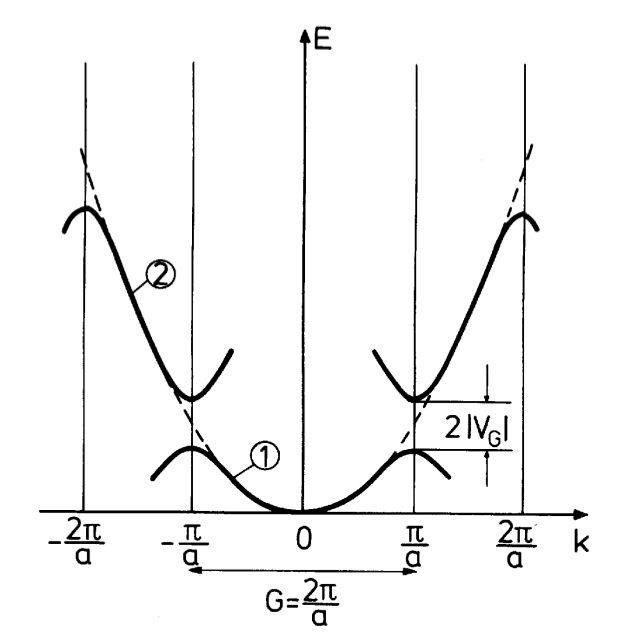
\includegraphics[width=0.5\textwidth]{pics/bloch}
  \end{captionbeside}
  \label{fig:bloch}
\end{figure}

Im Kristall gibt es nun Abweichungen von dem Modell. Zuerst einmal haben Kristalle 
endliche Ausdehnungen, sodass das zuvor als kontinuierlich angenommene 
Energiespektrum diskret ist. Zweitens haben die Elektronen eine Wechselwirkung. 
Diese ist gering im Vergleich zum Potenzial der Kerne, allerdings sorgt sie dafür, 
dass sich die erlaubten Energiewerte für Elektronen eines einzelnen Atoms aufspalten 
in $N$ sehr nahe beieinander liegenden Werten. Für große $N$ sind die erlaubten 
Energiewerte in dem so entstandenen \emph{Band} nahezu kontinuierlich, 
siehe Abb.~\ref{fig:baender1}. Pro Band können  
sich nach dem Pauliprinzip und unter Berücksichtigung des Spins maximal 2N Elektronen 
befinden. Geht die Temperatur gegen Null, so sind die Elektronen in der Konfiguration 
mit der niedrigsten möglichen Gesamtenergie angeordnet. Das oberste dann voll mit 
Elektronen besetzte Band wird als \emph{Valenzband} bezeichnet. Wird die Temperatur 
erhöht, so steht thermische Energie zu Verfügung. Die maximal Energie, die Elektronen 
im Mittel erhalten würden, wenn erlaubte Energiezustände vorhanden wären, wird als 
\emph{Fermienergie} bezeichnet. 
Liegt das Energieband über dem Valenzband unterhalb der Fermienergie oder hat sogar 
einen Überlapp mit dem Valenzband, so können Elektronen Enrgie aufnehmen und in dieses 
Band gelangen. Dort sind sie räumlich deutlich schwächer gebunden und können bei einem 
von außen angelegtem Feld in Richtung des Feldes driften. Daher wird das Band über dem 
Valenzband als \emph{Leitungsband} bezeichnet. Metalle sind deshalb elektrische Leiter, weil 
bei ihnen Leitungs- und Valenzband überlappen. Für das einwertige Natrium ist beispielsweise 
das oberste besetzte Band, das sich aus den 3$s$-Orbitalen zusammensetzt, nur halb besetzt. 
Für zweiwertige Metalle wie Magnesium überlappen sich Leitungs- und Valenzband. 
Bei Isolatoren liegt die Fermienergie niedriger als die untere Kante des Leitungsbandes. 
Die Elektronen können keine Energie eines angelegten Feldes aufnehmen und es kann kein 
Strom fließen. Bei Halbleitern ist die Fermienergie ab einer bestimmten Energie höher 
als die niedrigste Energie des Leitungsbandes. Daher ist ihre Leitfähigkeit 
temperaturabhängig. Siehe Abb.~\ref{fig:baender2}.\cite{demtroder2000experimentalphysik}\\ 

\newcommand{\picwidththeo}{0.48\textwidth}

\begin{figure}
    \centering
    \begin{subfigure}[b]{\picwidththeo}
        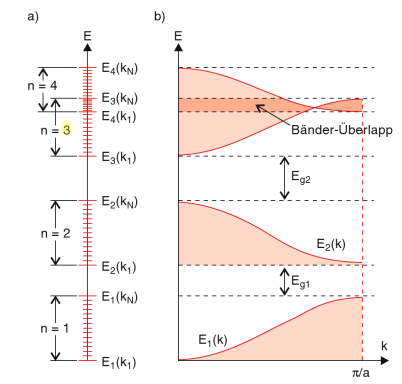
\includegraphics[width=\textwidth]{pics/baender1}
        \caption{Zur Entstehung der Energiebänder. Dargestellt ist die Aufspaltung der erlaubten 
Energiewerte von $N$ Elektronen im Kristall. 
(a) Eindimensionale Darstellung, 
(b) Darstellung von $E_n(k)$, die gestrichelte Linie ist die Grenze der 1. Brillouin-Zone;
aus \cite{demtroder2000experimentalphysik}}
        \label{fig:baender1}
    \end{subfigure}\qquad
    \begin{subfigure}[b]{\picwidththeo}
        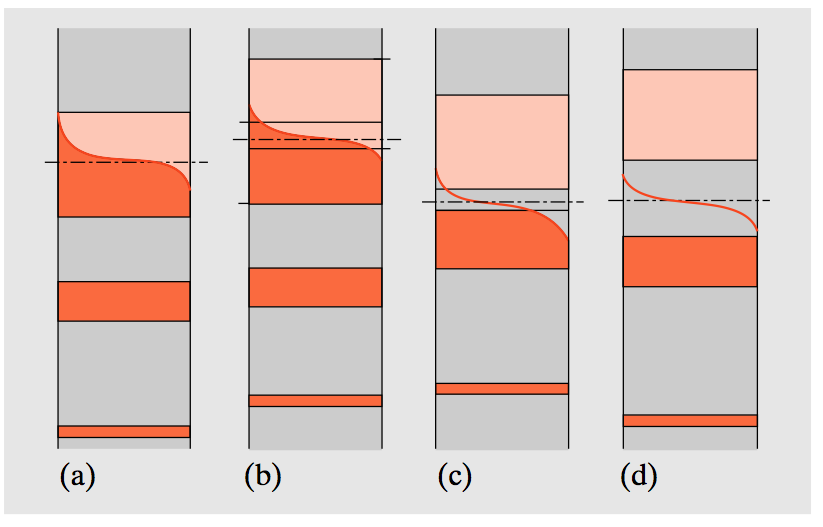
\includegraphics[width=\textwidth]{pics/baender2}
        \caption{Vereinfachte Darstellung des Bändermodells für 
(a) Metalle der ersten Hauptgruppe (Alkalimetalle), 
(b) Metalle der zweitern Hauptgruppe (Erdalkalimetalle), 
(c) Halbleiter (im leitfähigen Zustand)
(d) Isolatoren
aus \cite{vogel1997gerthsen}}
        \label{fig:baender2}
    \end{subfigure}
    \caption{Schemata zum Bändermodell}\label{fig:baender}
\end{figure}



\subsection{Grundlagen der Festkörperoberflächen}
Das zuvor angenommen, unendlich ausgedehnte, periodische Kristallgitter spielt 
bei der Untersuchung der Oberflächen nur noch eine untergeordnete Rolle – 
schließlich ist eine Oberfläche zunächst einmal eine Abweichung dieser 
Eigenschaft. Im Allgemeinen kann es Abweichungen in null, ein, zwei oder drei 
Dimensionen geben. Letztere sind Abweichungen der unterliegenden Baustruktur, 
die zum Teil eine Mosaikstruktur bilden, die sich auch auf größere Skalen 
erstrecken. Zweidimensionale Strukturen tauchen als großflächige 
Überstrukturen oder kleinere Facetten auf. Eine Kategorisierung verschiedener 
Oberflächen wird von Henzler und Göpel \cite{henzler1991oberflachenphysik} 
gegeben (Abb.:~\ref{fig:oberflaeche}).
In jedem Fall erfahren die Atome der Oberfläche nicht mehr das 
regelmäßige Potential von allen Seiten. Dies resultiert je 
nach Art als Oberflächenrelaxation oder -rekonstruktion. 
Ersteres bezeichnet lediglich eine globale Verschiebung der oberen Schicht 
gegen die Basis, beispielsweise normal oder lateral, wobei die Symmetrien 
der Oberfläche nicht verändert werden und sich die freie Energie verringert. 
Dieser Effekt wird bei den meisten Metallen beobachtet \cite{oura2003surface}. 
Abb. \ref{fig:Ag(110)} zeigt beispielsweise die relaxierte Oberfläche von Silber 
auf der (110)-Fläche.
Bei der Oberflächenrekonstruktion bilden sich meist größere Einheitszellen als die 
des darunter liegenden Kristalls. Bei Halbleitern hängt das oft damit zusammen, 
dass die Anzahl nicht abgesättigter Bindungen minimiert wird, so beispielsweise 
bei Silizium entlang der (100)-Fläche, bei der nach gedanklichem Aufspalten zwei 
Bindungen frei wären. Je zwei Atome verbinden sich zu sog. Dimeren, wobei die 
Oberfläche räumlich verzogen wird und sich volle bzw. leere Reihen mit einer 
Höhe von bis zu fünf Schichten und über große Entfernungen bilden 
\cite{chadi1979atomic}. Die bereits in der historischen Einleitung gezeigte 
Si-Oberfläche entlang der 
(111)-Ebene zeigt ebensfalls eine Oberflächenrekonstruktion, allerdings mit 
deutlich anderen Mustern. Die kubisch-flächenzentrierten Edelmetalle der 
6.~Periode, Ir, Pt und Au bilden als Ausnahme unter den Metallen ebenfalls 
Oberflächenrekonstruktionen, die sog. \emph{missing row}-Konstruktion, 
wie weiter unten bei der Beschreibung von Gold verdeutlicht wird 
\cite{kittel2013einfuhrung}. 

\begin{figure}[!t]
  \begin{captionbeside}[]{Rastertunnelkikroskop-Aufnahme mit atomare Auflösung einer reinen 
Silberoberfläche entlang der (110)-Fläche. Zu erkennen ist, dass die Oberfläche 
lediglich relaxiert ist, und Rekonstruktion stattfindet. 
Aus \cite{kahn:stm_images}.}[r]
    
\includegraphics[width=0.5\textwidth]{pics/Ag(110)_clean}
  \end{captionbeside}
  \label{fig:Ag(110)}
\end{figure}

Zur mathematischen Beschreibung regelmäßiger Überflächen werden die Gittervektoren 
aus dem Ortsraum benutzt, die in der Oberfläche liegen. Ausreichend sind meistens 
jene aus der obersten Atomschicht. Die Atome befinden sich dann an den Positionen 
\begin{equation}
    \mathbf{r} = m_1 \mathbf{a_1} + m_2 \mathbf{a_2},
\end{equation}
wobei nach Konvention $|\mathbf{a_1}| \le |\mathbf{a_2}|$ und 
$\gamma = \angle (\mathbf{a_1}, \mathbf{a_2}) > 90 \deg$ der Winkel zwischen den 
beiden Vektoren ist. Da die Atome in einer Ebene liegen, ist die Anzahl möglicher 
Anordnungen, die sog. Bravais-Netze, deutlich kleiner als für einen 3D-Kristall. 
Es gibt genau fünf, wie in Abb.~\ref{fig:Bravais} gezeigt 
\cite{henzler1991oberflachenphysik}.
Zur vollständigen Beschreibung fehlen dann allerdings noch die Angaben zur Lage 
der Oberflächenatome relativ zur darunter befindlichen Basis. 

Zur Beschreibung der Oberfläche wird zuerst die ideale Oberfläche angenommen, 
die sich aus dem darunter liegenden Kristallgitter ergäbe, und deren Vektoren mit
$|\mathbf{a_1}| \le |\mathbf{a_2}|$ bezeichnet werden. Die tatsächliche Struktur, 
soweit periodisch, kann dann als Verhältnisse $\frac{\mathbf{a_1}}{\mathbf{b_1}}$, 
$\frac{\mathbf{a_1}}{\mathbf{b_1}}$ und Winkel zwischen Basis und Oberfläche angegeben 
werden. Zusammen mit der Millerschen Schreibweise für die Kristallfläche der Basis 
ergibt sich so eine kompakte Schreibweise, z.~B. 
$\mathrm{Si}(111)(\sqrt{3} \times \sqrt{3}) \mathrm{R} 30 \deg$. 
Ist diese Schreibweise ungeeignet aufgrund fehlender Symmetrien, so kann eine 
Matrixschreibweise benutzt werden. Sind die Einträge ganze Zahlen, so liegen die 
Atome der Oberfläche direkt auf der Basis. Bei rationalen Zahlen gibt es auch 
zwischen den Basisatomen Oberflächenatome, während bei irrationalen Zahlen die 
Oberfläche quasi unabhänging von der Basis gesehen werden muss. Sie wird dann auch 
als inkommensurabel bezeichnet\cite{henzler1991oberflachenphysik}.

\begin{figure}
    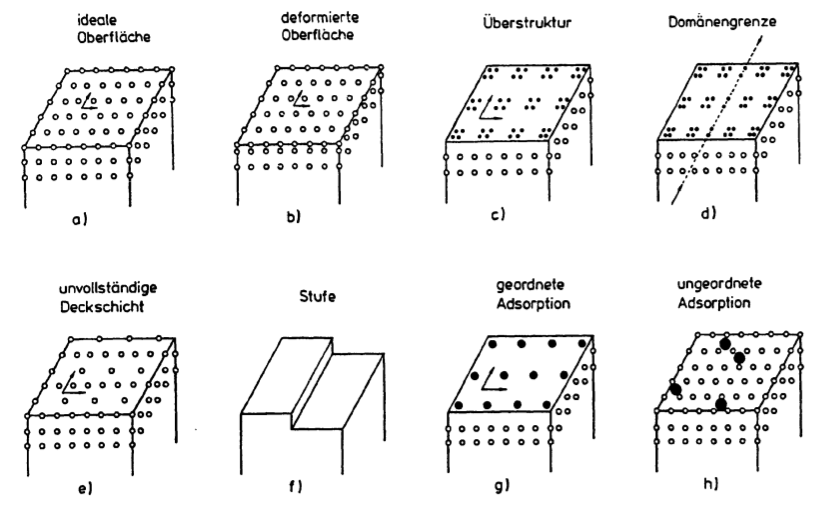
\includegraphics[width=1.0\textwidth]{pics/oberflaechenstruktur}
    \caption{Die ideale Oberfläche und einige mögliche Oberflächenstrukturen. 
Die ideale Oberfläche entspricht einer Gitterebene im Kristall, die defomierte 
Oberfläche entsteht durch Relaxation (hier in normaler Richtung) und wird bei den 
meisten Metallen beobachtet, während die Überstruktur ein Resultat der Rekonstruktion 
ist und z. B. bei Halbleitern oder Gold zu beobachten ist. 
Aus \cite{henzler1991oberflachenphysik} }
\label{fig:oberflaeche}
\end{figure} 
\begin{figure}
  \begin{captionbeside}{Bravais-Gitter zur Oberflächenstrukturbeschreibung. Die 
kleinstmöglichen Zellen sind in den unteren drei Gittern mit $\underline{a}_2^p$ 
beschriftet. 
Aus \cite{henzler1991oberflachenphysik}. }[r]
    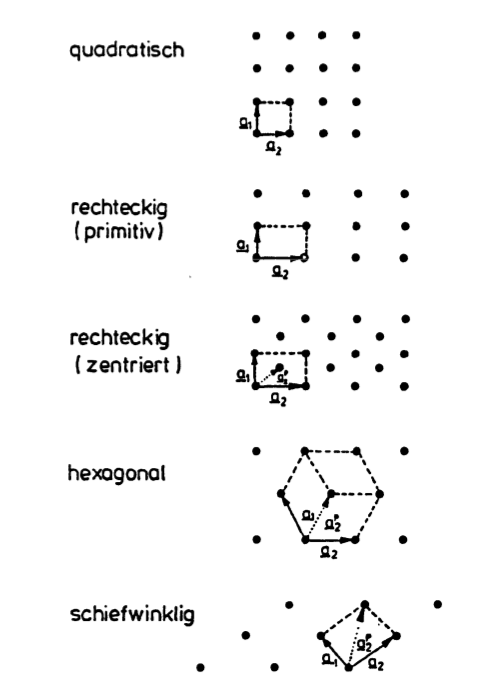
\includegraphics[width=0.5\textwidth]{pics/Bravais}
  \end{captionbeside}
  \label{fig:Bravais}
\end{figure} 


\subsection{Struktur von Graphit, Gold und $\mathrm{MoS_2}$}
Die Kristallstruktur von Graphit zeichnet sich vor allem durch seine Schichtenstruktur 
aus. Die Kohlenstoffatome sind in den aus kovalent gebundenen Sechsecken bestehenden 
Basalebenen oder Graphenschichten deutlich fester aneinander gebunden (4.3 eV), als 
an solche aus benachbarten Schichten (0.07 eV). Daher ist Graphit entlang dieser Linien 
sowohl mechnisch deutlich stabiler als auch sehr viel leitfähiger (für Wärme und 
elektrischen Strom). Die Unterschiede in der Bindungsenergie spiegeln sich auch in den 
Abständen wider: So sind nächsten Nachbarn innerhalb einer Schicht nur $0.142\mathrm{nm}$ 
entfernt, während die Schichten $0.335\mathrm{nm}$ auseinander liegen.  
Graphit tritt nicht nur in zueinander korrlierten Schichten auf, 
sondern auch unkorrliert (sog. turbostratischer Kohlenstoff). Die hier untersuchte Form 
ist jedoch regelmäßig - die Winkelabweichung für das verwendete HOPG (highly orientated 
pyrolytic graphite) beträgt weniger als $1 \deg$ \cite{mcnaught2000iupac}. Diese 
synthetische Form des Graphit wird auf Grund von ihrer Regelmäßigkeit und Reinheit 
heute zur Kalibrierung von Rastertunnelmirkoskopen verwendet \cite{lapshin1998automatic}. 
Es liegen in der Schichtung jedoch nicht alle Atome übereinander, sondern lediglich 
jedes zweite aus jedem Sechseck (siehe Abb.~\ref{fig:graphite}). 
Dadurch kommt es an der Oberfläche zu einem oft beobachteten 
Effekt: Anstatt sämtliche Atome der Sechsecke zu beobachten, taucht nur die Hälfte auf 
den STM-Bildern auf. Erklärt wird das dadurch, dass die Elektronendichte in der 
Fermienergie für Atome mit Nachbarn darunter höher liegt als bei solchen ohne
\cite{zeinalipour2008new}. Selloni~et~al.~\cite{Sellino1985} berechneten den Abstand 
der Atome mit bzw. ohne direkten Nachbarn in der Schicht darunter mit $0.15 \AA$. 

\begin{figure}
    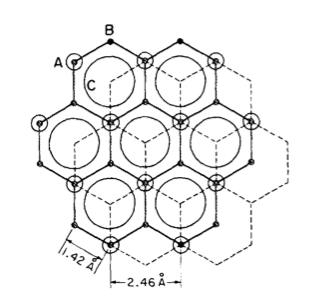
\includegraphics[width=0.7\textwidth]{pics/graphite}
    \caption{Hexagonale Oberflächenstruktur von Graphit. An den umkreisten Orten (A) 
liegen jeweils Atome aus der ersten und der zweiten Schicht übereinander, bei den 
übrigen (B) nicht. Bei STM-Aufnahmen sind fast ausschließlich die Atome mit Nachbarn 
zu erkennen, da hier Elektronen nahe der Fermienergie räumlich weiter oben liegen. 
Aus \cite{park1986tunneling}}
    \label{fig:graphite}
\end{figure} 

Gold ist als kubisch-flächenzentriertes Kristallgitter aufgebaut. Die Gitterkonstante 
beträgt $407.82\mathrm{pm}$\cite{ohring1995engineering}. Im Gegensatz zum Graphit 
treten jedoch beim Gold enorme Veränderungen der Oberflächenstruktur gegenüber der 
darunter liegenden Basis auf. Auf einer (110)-Fläche wurde die Bildung von 
(111)-Facetten beobachtetet, die Kanälevon meistens zwei bis vier Schichten Tiefe 
formen. Gleichzeitig ist die Oberfläche von Stufen gekennzeichnet, die sowohl parallel 
als auch normal zu den Kanälen verlaufen, siehe Abb. \ref{fig:Au(110)_channels}. Die Darstellung 
der Oberfläche mit dem Rastertunnelmikroskop ist auf Grund der metallischen Struktur 
deutlich schwieriger als bei Halbleitern, da die Elektronen aus dem Leitungsband kaum 
räumlich lokalisiert sind. 

\begin{figure}
    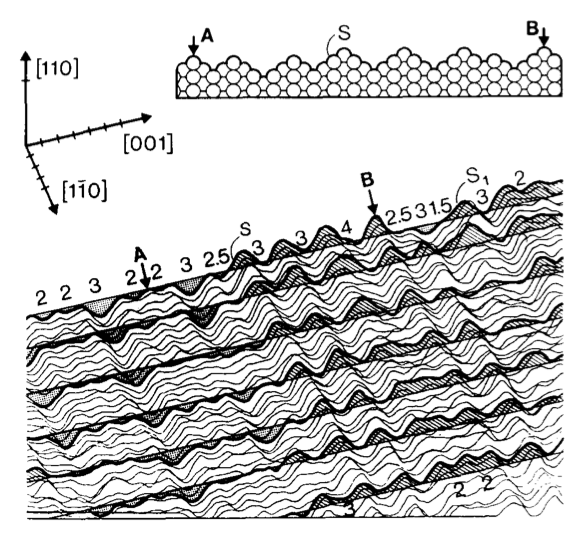
\includegraphics[width=0.6\textwidth]{pics/Au(110)_channels}
    \caption{Rastertunnelmikroskop-Aufnahmen von Gold(110)-Oberfläche mit 
Rekonstruktion. Die Geraden verdeutlichen die abschüssige Terassenstruktur, die 
Nummern die Tiefe der Kanäle (in Vielfachen der Ebenenabstände). Bei $\mathrm{S}$
und $\mathrm{S_1}$ befinden sich Stufen mit Höhe einer Atomlage. An den Kristallaxen 
ist der Maßstab gekennzeichnet: ein Schritt entsprechen 5 \AA. Über der Aufnahme 
deutet ein schematischer Querschnitt die Struktur der Kanäle an. 
Aus \cite{binnig1983111}.}
    \label{fig:Ag(100)}
\end{figure} 

Molybdänit ($\mathrm{MoS_2}$, auch Molybdän(IV)-sulfid) ist ein Halbleiter mit 
hexagonalem Kristallgitter der Raumgruppe $\mathrm{P \, 6_3/mmc}$. Ähnlich 
dem Graphit gibt es eine schichtartige Struktur, auch hier können die Schichten 
relativ leicht gegeneinander verschoben werden. Die Gitterparameter sind mit 
$a = 3.161 \AA$ sowie $c = 12.295 \AA$ angegeben, siehe
Abb.~\ref{fig:MoS2_structure} \cite{schrocke1981mineralogie}. 
Auf Gund der Schichtstruktur findet $\mathrm{MoS_2}$ als 
Schmiermittel Verwendung und kann wie Graphen als einatomige Schicht isoliert 
werden, sodass es mögliches Transitormaterial gehandelt wird 
\cite{mak2010atomically}. 

\begin{figure}
  \begin{captionbeside}{Gitterstruktur von $\mathrm{MoS_2}$, Ausschnitte aus drei übereinander 
liegenden Schichten mitsamt Koordinationspolyedern. Für die Abstände gilt 
$a_1 = a_2 = a_3 = 3.161\AA =: a$ und $c_0 = 12.295\AA$. 
Aus \cite{schrocke1981mineralogie}.}[r]
    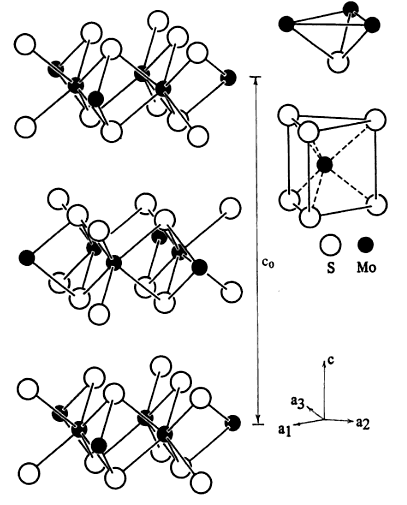
\includegraphics[width=0.5\textwidth]{pics/MoS2_structure}
  \end{captionbeside}
  \label{fig:MoS2_structure}
\end{figure} 

\subsection{Statistische Analyse von Höhendaten}
\usetikzlibrary{decorations.pathreplacing}
Ausserhalb der gewöhnlichen statistischen Analyse, die wir
hier als bekannt voraussetzen, führen wir hier weitere Werkzeuge
ein, die sich spezial für die Analyse rauer Oberflächen bzw. 
Gitterstrukturen als nützlich erweisen\cite{gwyddion}. Zunächst
gehen wir davon aus, dass uns die Mikroskopiedaten als 
$N \times M$ Vektorfeld vorliegen (N Zeilen und M Spalten der
Matrix der Bilddaten, ). Die tatsächliche Fläche der Daten
nennen wir nun $L_x \times L_y$, wobei 
wir ObdA nehmen nun annehmen, dass die Abstände
zwischen den Datenpunkten $\Delta$ betrage 
(siehe Abbildung~\ref{fig:stat1}). 

\begin{figure}
\begin{tikzpicture}
\draw[step=1cm,gray,very thin] (-1,-1) grid (5,6);
\draw  (-1,-1) -- (5,-1) -- (5,6) -- (-1,6) -- (-1,-1);
\draw [<->] (-1,6.5) node [left]{$M$} -- (-1,-1) 
-- (5.5,-1) node [right] {$N$};
\draw [decoration={brace,mirror,raise=5pt},decorate]
(-1,-1) --  node[below=10pt]{$L_x$}(5,-1); 

\draw [decoration={brace,raise=5pt},decorate]
(-1,-1) --  node[left=10pt]{$L_y$}(-1,6); 

\end{tikzpicture}
\caption{Das Vektorfeld der Mikroskopiedaten besteht aus 
$N \times M$ Höhendaten aus $\mathbb{R}$, wobei die tatsächliche 
Fläche $L_x \times L_y$ beträgt.}
\label{fig:stat1}
\end{figure}
Wir betrachten nun 
die statistischen Eigenschaften der Zufallsvariablen $\xi(x,y)$. 
Die Wahrscheinlichkeitsdichte $\rho(x,y,z)$ für eine 
bestimmte Höhe $z$ ergibt sich numerisch
durch die Extrapolation der einzelnen Datenpunkte mit der Normierung:
\begin{equation*}
\int \rho(x,y,z) dx dy dz = 1
\end{equation*}
Nun lässt sich mithilfe von $\rho$ die 2-Punkt-Funktion
(2-point function) definieren:
\begin{equation}
w(\tau_x=x_1-x_2, \tau_y=y_1-y_2,z_1,z_2) = \rho(x_1,y_1,z_1)
\rho(x_2,y_2,z_2)
\end{equation}
Wobei wir die Abstände $\tau_x=x_1-x_2$ und $\tau_y=y_1-y_2,z_1,z_2$
definiert haben.
\subsubsection{Fourier Transformationen}
Sei nun ganz allgemein die Fouriertransformation eingeführt:
\begin{align}
f(x) &= \int_{-\infty}^{\infty} F(k)\exp(2\pi i kx)dk\\
F(k) &= \mathcal{F}_x\left [f(x)\right ](k) =
\int_{-\infty}^{\infty} f(k)\exp(-2\pi i kx)dx
\end{align}
Mit den (nur den wichtigsten) Eigenschaften:
\begin{align}
&\mathcal{F}\left [a f(x) + b g(x)\right ]
    = a F(k) + b G(k) 
    &\mbox{ (Linearität) }\\
&\mathcal{F}\left [f(x) * g(x)\right ](k)
    = \mathcal{F}\left [f(x)\right ]\mathcal{F}\left [g(x)\right ]
    \! &\mbox{ (Faltungseigenschaft) }\\
&\mathcal{F}_k\left [\left | F(k) \right |^2\right ](x)
   =  \int_{-\infty}^{\infty}\bar{f}(\tau)f(\tau + x) d\tau 
   &\mbox{ (Wiener-Khinchin Theorem) }
\end{align}
In der letzten Eigenschaft
bedeutet $\bar{f}$ die komplexe Konjugation von $f$.
Die Definitionen sind nun für die x-Richtung ausgeführt worden,
sie funktionieren jedoch analog im $2D$ Fall, also mit dem Tuple
$(x,y)$. 
Um das Leistungsspektrum berechnen zu können, führen wir 
nun die Autokorrelationsfunktion ein:
\begin{align}
    G(\tau_x,\tau_y) &=\int\int z_1 z_2 w(\tau_x,\tau_y,z_1,z_2) dz_1 dz_2 \mbox{ (Autokorrelationsfunktion) }\\
&= \int\int \xi(x_1,y_1)\xi(x_1+\tau_x,y_1+\tau_y)dx_1dy_1
\end{align}
Diese Funktion lässt sich nun auch diskret berechnen:
\begin{equation}
    G(m,n)=\frac{1}{(N-n)(M-m)}\sum_{l=1}^{N-n}\sum_{k=1}^{M-m}z_{k+m,l+n}z_{k,l}
\end{equation}
wobei $m=\tau_x/\Delta_x$ und $n=\tau_y/\Delta_y$.
Wie wir sehen, fügt sich nun die Vorarbeit nun zusammen und 
aus den unseren gemessenen diskreten Höhendaten lässt  
sich nun direkt die Autokorrelationsfunktion
berechnen. 
Um nun eine qualitative Aussage über die Verteilung der Moden
treffen zu können, berechnen wir das Leistungsspektrum (mithilfe
des Wiener-Khinchin Theorems):
\begin{align}
    W(K_x,K_y)=\frac{1}{4\pi}\int\int G(\tau_x,\tau_y)\exp(-i(K_x\tau_x+K_y\tau_y)) d\tau_xd\tau_y
\end{align}
Diese lässt sich wieder analog zur Autokorrelationsfunktion
für diskrete Werte berechnen. Wenn eine isotrope Struktur
vorläge, würde es sich nun anbieten, über die Fläche zu 
integrieren. Da dies bei unseren Proben nicht der Fall ist,
werden wir dies hier nicht weiter ausführen.\\

In der numerischen Analyse wird nun die ``Schnelle''
Fouriertransform (engl. \textit{Fast Fourier Transform, FFT})
berechnet. \\Da wir die Integraltransformationen
bei einem begrenzten und
nicht unendlichen Datensatz mit der
diskreten Fourier Transformation (DFT)
approximieren müssen, implizieren wir zyklische Randbedingungen:
\begin{align}
 &f(n) = \frac{1}{N}\sum_{n=0}^{N-1}{\exp(2\pi i \frac{kn}{N})f(k) }\\
 &F(k) = \sum_{n=0}^{N-1}{\exp(-2\pi i \frac{kn}{N})f(n) }
\end{align}
Da die realen Datensätze diese zyklischen
Randbedingungen nicht aufweisen, müssen
die Ränder des Datensatzes ``unterdrückt'' bzw. transformiert
werden. Generell wird dazu eine Fensterfunktion (\textit{Window
function}) verwendet, welche mit dem Signal gefaltet wird und
somit die bei der FFT auftretenden Randeffekte zu unterdrücken 
sucht (siehe Abbildung~\ref{fig:stm2}). 
Dabei sind verschiedene Windowfunctions
denkbar (siehe Abbildung~\ref{fig:windowing-fft},
welche über verschiedene
Güten verfügen und an die Eigenschaften
des Signals angepasst werden müssen.
\begin{figure}
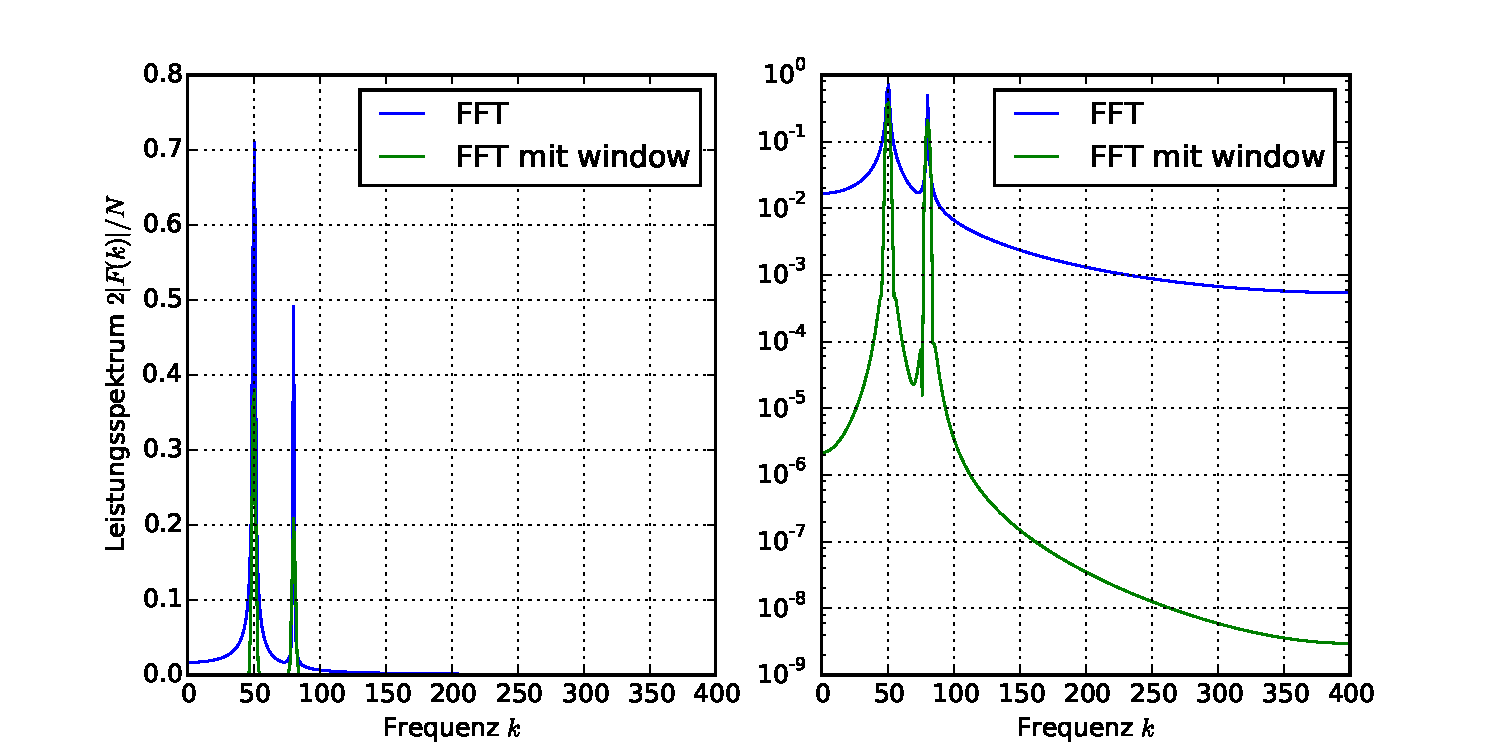
\includegraphics[width=17cm]{pics/stm2}
\caption{Hier berechnen wir numerisch die diskrete
    Fouriertransformation (FFT) des Signals  
$f(t)=\sin(2\pi \omega_1 t) + 0.5 \sin(2\pi \omega_2 t)$ mit den 
Frequenzen $\omega_1 = 50$ und $\omega_2 = 80$, jeweils mit
der Windowfunction \textit{blackman} und ohne. 
Die Berechnung erfolgte mit $N=600$ mithilfe der numerischen
Bibliothek \textit{numpy/scipy} in Python\cite{scipy_reference}.
Der Sourcecode dazu befindet sich im Anhang.
Wie aus den Diagrammen ersichtlich wird, bildet die windowfunktion
\textit{blackman} zusammen mit der FFT
die  beiden Frequenzen $\omega_1$ und $\omega_2$ viel besser ab
als die FFT alleine. Dies ist auch wichtig bei der Analyse der
Datenpunkte aus dem RTM, welche auch nur in diskret vorliegen.
}
 \label{fig:stm2}
\end{figure}

\begin{figure}
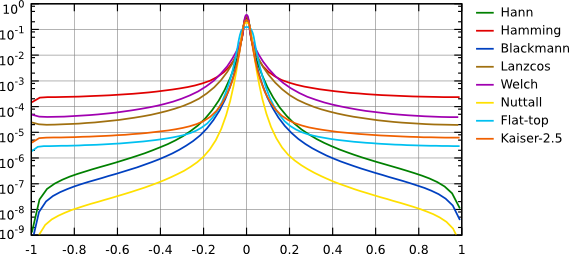
\includegraphics[width=17cm]{pics/windowing-fft}
\caption{Verschieden mögliche Windowfunktionen\cite{gwyddion}.
Die verschiedenen Funktionen unterscheidenen sich in ihrer
sogenannten \textit{Bandbreite}, das bedeutet, dass es keine
ideale Windowfunktion gibt, sondern dass jene an das Signal
angepasst werden muss. } 
\label{fig:windowing-fft}
\end{figure}

\subsubsection{Reziprokes Gitter und Fouriertransformationen}
Den Reziproken Raum (auch k-Raum genannt) erhält man durch die
Fouriertransformation des Ortsraumes. Somit erhalten wir durch
die Fouriertransformation des Gitters die erste Brillouin-Zone
des Reziproken Gitters. Deshalb bietet es sich an, mithilfe
des Leistungsspektrums der 2D-Fouriertransformation der 
Mikroskopiedaten die Gittereigenschaften der Probe zu analysieren
(Siehe Quelle \cite{kelty1991scanning}. In der Quelle wird zwar  
nicht explizit auf Methode eingegangen, sie wird allerdings
verwendet, um die Superstruktur von $KHgC_4$ in verschiedenen
Formen zu analysieren, siehe Abbildung~\ref{fig:powerspec}). 
\begin{figure}
    \begin{captionbeside}[]{Abbildungen aus \cite{kelty1991scanning}.
(a) Es handelt sich um eine 100x100 $\r{A}^2$ Rastertunnelmikroskopiebild
von $KHgC_4$ mit einem $8.9 \r{A}$ Gitterperiodenabstand.
(b) das 2DFT Power Spektrum, welches deutlich die Symmetrie des 
Supergitters und seine Orientierung zeigt.} 
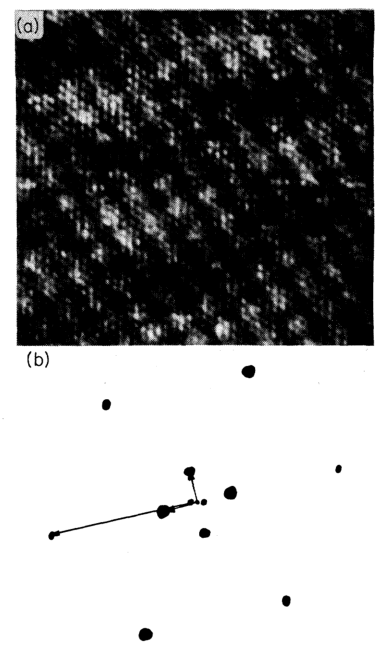
\includegraphics[width=6cm]{pics/powerspec}
\end{captionbeside}
\label{fig:powerspec}
\end{figure}



\section{Durchführung des Versuchs}
In Abbildung~\ref{fig:stm1} sehen wir das RTM, welches in der
folgenden Versuchsdurchführung verwendet wurde. Es handelt sich
um das Modell \textit{easyScan 2 STM, Version 1.6} welches von 
der Firma \textit{Nanoscience Instruments, Ink.} vertrieben wird.
Laut der Beschreibung des Herstellers 
bilden hunderte \textit{easyScan 2 STMs} einen
\textit{unersetzlichen} Bestandteil in der Lehre von Physik,
Chemie und Materialwissenschaften, werden aber auch in der
Forschung und Entwicklung eingesetzt. Anwendung findet das RTM
in der Spektroskopie sowie in der Grundlagenforschung.
In unserem Versuch spielt das easyScan 2 STM insofern eine Rolle,
dass es ohne weitere Zwischeninstanzen direkt die gemessen
Abstände in ein Bild auf dem Computer sendet. Diese Bilder
enthalten schon alle für den Versuch notwendigen Informationen,
die Parameter können auch direkt von dem bereitgestellten Programm
konfiguriert werden. Der Wandel vom ersten RTM, in dem die Dämpfung
noch von Supraleitenden Magneten und einer Vakuumkammer hergestellt
werden musste, zum diesem Modell und diese Fortschritt kommt uns
in unserem FP zu Gute. Die Spezifikationen des Modells 
(Ausschnitt, entnommen aus dem beiliegendem Handbuch):\\
\begin{table}[h]
\begin{tabular}{| l | p{7cm} |}
\hline
  Größe des Controllers, Gewicht: & 470x120x80 mm / 2.4 Kg\\ \hline
  Leistung & 90- 240 V~/ 30 W 50/60 Hz \\ \hline
  Rastergeschwindigkeit & Bis zu 60ms pro Linie mit 128 Datenpunkten  pro Linie \\ \hline
Rasterfläche & bis zu 2048x2048 Punkten \\ \hline 
Darstellungsmöglichkeiten: & Liniengraph, Farbplot und 3D Perspektive \\ \hline
Abbildungsmodi & Konstante Stromstärke (\textit{Constant Current}),
konstante Höhe (\textit{Constant Height}) \\ \hline
Maximale Auflösung in Z/ XY & 3pm/ 7.6pm \\ \hline
Maximaler Rasterumfang in Z/ XY & 200nm/ 500nm  \\ \hline
Maximale Probengröße & 10mm Durchmesser \\ \hline
Spitzenspannung & max. $\pm 10V$ in 5mV Schritten \\ \hline
\end{tabular}
\caption{Spezifikationen des Modells \textit{easyScan 2 STM}}
\label{tab:STM}
\end{table}

\begin{figure}
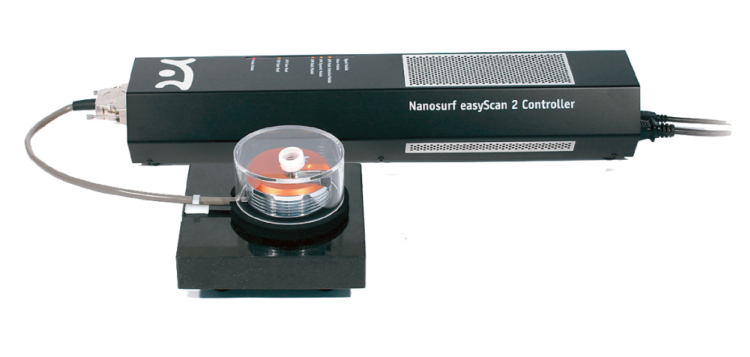
\includegraphics[width=14cm]{pics/stm1}
\caption{Photographie des verwendeten RTMs \textit{easyScan 2
STM Version 1.6} (entnommen aus Webseite des Herstellers)} 
 \label{fig:stm1}
\end{figure}

Da die Messaparatur für unseren Versuch schon aufgebaut worden
war und nicht modifiziert werden sollte, werden wir hier nicht
auf die einzelnen Komponenten des \textit{easy Scan 2 STM} Systems
eingehen, sondern nur die für unseren Versuch relevanten 
Bauteile beschreiben.
\subsection{Versuchsaufbau}
In Abbildung~\ref{fig:Rasterkopf} ist der Rasterkopf ds RTMs zu
sehen. Über den Probenhalter mit dazugehörigem Fixierungsmagneten
wird die Probe selbst angebracht; an den Spitzenhalter mit
Klammer die Spitze aus Platin-Iridiumdraht, 
welche wir für die Messungen selbst herstellt haben (siehe
Abbildung~\ref{fig:prepare_tip} und Abbildung~\ref{SEM_tip_picture}).
Der Probehalter stellt einen Zylinder dar, an dessen Kopf mithilfe
eines Magneten die Probe, welche im Idealfall auf einer dafür
passenden, ebenfalls magnetischen Schablone angebracht ist, 
befestigt wird, nachdem die Spitze angebracht wurde. 
Das Anbringen der Spitze erfolgt mit dafür passenden Zangen,
indem die Klammer angehoben, die Spitze eingelegt und mit
der Klammer fixiert wird.

\begin{figure}
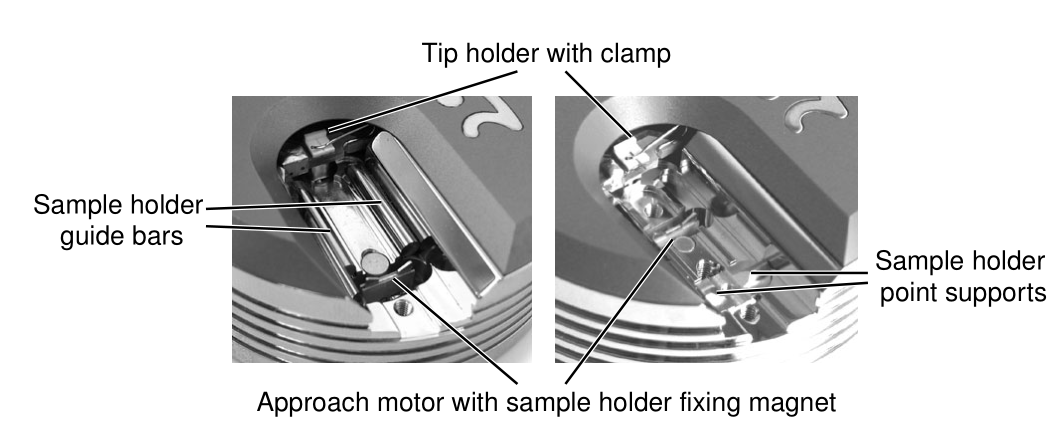
\includegraphics[width=14cm]{pics/rasterkopf}
\caption{Rasterkopf des RTMs \textit{easyScan 2
STM Version 1.6} (entnommen aus Webseite des Herstellers)
Zu sehen ist der Probenhalter (\textit{Sample holder}) mit dazu
gehörendem Annäherungsmotor (\textit{Approach motor} sowie
dem Fixierungsmagneten ({Fixing Magnet}), sowie dem Spitzenhalter
mit Klammer (\textit{Tip holder with clamp}). Die Funktionsweise
wird im Text beschrieben.}
 \label{fig:Rasterkopf}
\end{figure}

\begin{figure}
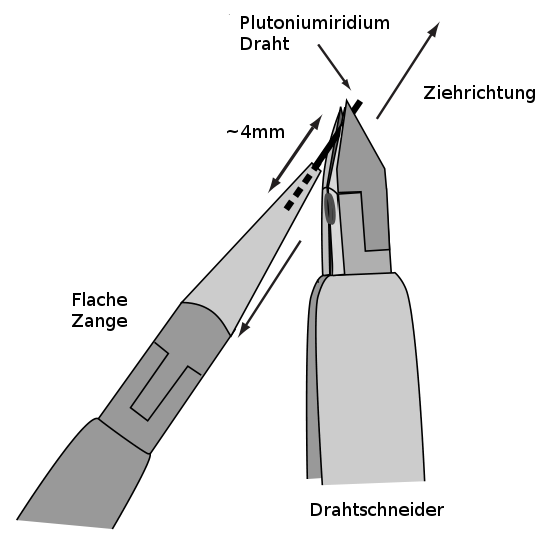
\includegraphics[width=10cm]{pics/prepare_tip2}
\caption{Vorbereitung des Drahtes. 1) Zunächst sollten die
zur Herstellung der Spitze notwendigen Werkzeuge mit Ethanol
gereinigt werden, von nun an sollte nur der Draht damit berührt 
werden. 2) Nun sollte der zu verknappende Draht mit den Zangen
gehalten werden, 3) dem Drahschneider umschlossen, aber nicht
abgezwickt, 4) in die angegebene Richtung \textbf{gezogen}, 5)
und endlich \textbf{abgerissen} werden, mit dem Ziel eine 
einatomige Spitze zu erzeugen (siehe Abbildung~\ref{fig:SEM_tip_picture})}
 \label{fig:prepare_tip}
\end{figure}

\begin{figure}
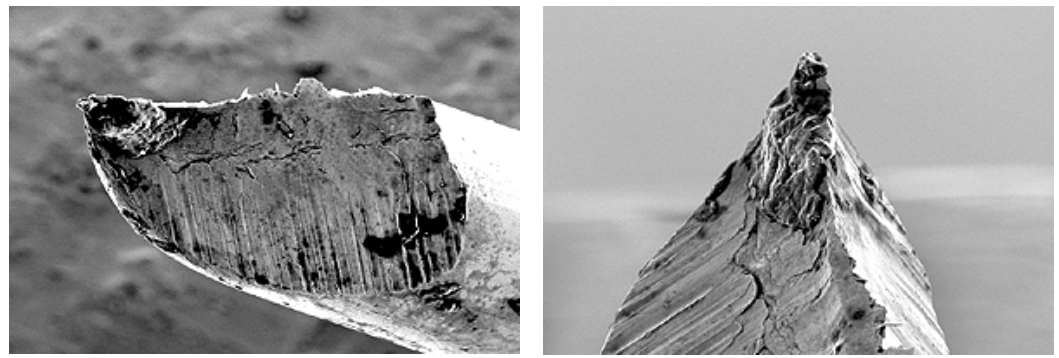
\includegraphics[width=10cm]{pics/SEM_tip_picture}
\caption{Das in Abbildung~\ref{fig:prepare_tip} beschriebene
Verfahren hat zum Ziel, eine möglichst präzise Spitze herzustellen.
Hier eine \textit{Scanning Electron Microskope} Abbildung
aus der Bedingungsanleitung des RTMs 
einer solchen hergestellen, idealen Spitze. Wie deutlich erkennbar
ist, verjüngt sich die Spitze nach oben und bietet so unter 
Umständen die Möglichkeit, eine einatomige Tunnelverbindung
mit der Probe einzugehen.}
 \label{fig:SEM_tip_picture}

\end{figure}
\subsection{Durchführung der Messungen}
Sobald die Spitze angebracht und die Probe eingeführt wurde, 
kann der Annäherungsprozess der Spitze zu der Probe beginnen. 
Zunächst kann manuell mit einer groben Steuerung die Spitze
(visuell) so nah wie möglich an die Probe herangebracht werden.
Dabei ist es von Vorteil, wenn diese schon zu Beginn recht nahe
aneinander liegen. Danach startet man den automatischen
Annäherungsprozess,
der die Spitze solange mit einer jeweils eingestellten
Geschwindigkeit der Probe annähert, bis ein erster Tunnelstrom
(in der Regel 1 nA)
zwischen der Probe und der Spitze fließen kann.  
Dieser Annäherungsversuch verfügt über verschiedene Modi:
\begin{itemize}
    \item \textbf{\textcolor{orange}{orange}}:
            Der Annäherungsversuch ist noch
            nicht abgeschlossen
    \item \textbf{\textcolor{red}{rot}}: 
            Der Annäherungsversuch ist in dem Sinne
            gescheitert, dass die Spitze mit der Probe kollidiert
            ist und womöglich Schaden erlitten hat. 
    \item \textbf{\textcolor{green}{grün}}: 
            Der Annäherungsversuch
            wurde ohne Fehlermeldungen
            abgeschlossen und ist vermutlich geglückt;
            der Tunnelstrom fließt wie vorgegeben.
\end{itemize}
Der erste Annäherung genügt in der Regel nicht, die Probe
mit der gewünschten Auflösung betrachten zu können. Deswegen muss
sukzessiv die Distanz 
durch weitere Annäherungen verkleinert werden,
unter jeweils niedrigerer
Tunnelspannung und veringerter Annäherungsgeschwindigkeit, 
ohne dass dabei die Spitze mit der Probe kollidiert.
Wenn nun die Annäherung erfolgt ist, kann die Abrasterung
der Probe beginnen. Die Qualität des Kontakts zwischen Probe
und Spitze kann nun anhand verschiedener Kriterien beurteilt werden,
darunter die der Spitze umgebende Höhenlinie (siehe
Abbildung~\ref{fig:topography}).
\begin{figure}
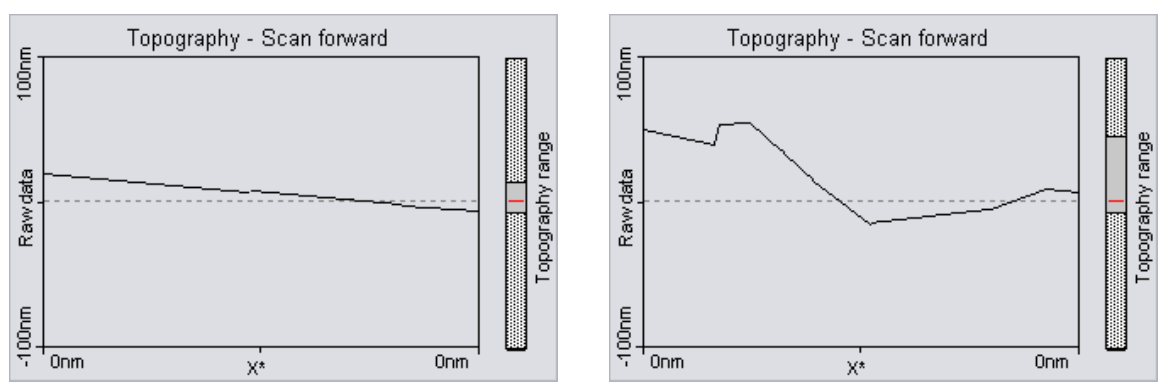
\includegraphics[width=14cm]{pics/Topography}
\caption{Screenshot aus dem Programm. Links zeigt eine 
Topographische Linie für einen guten Kontakt, während die
rechte ``nervöse'' Linie aufgrund ihrer Nichtlinearität
einen schlechten Tunneling Kontakt
andeutet, was auf eine zu stumpfe oder instabile Spitze
zurückgeführt werden kann.}
 \label{fig:topography}
\end{figure}
Wenn nun eine erfolgreiche Abrasterung mit zufriedenstellender
Auflösung vorliegt, kann ein Ausschnitt der Abrasterung
vergrößert werden, dieser Auschnitt wird dann erneut abgerastert
(sofern die technisch mögliche Auflösung nicht überschritten wird,
siehe Tabelle~\ref{tab:STM} auf Seite~\pageref{tab:STM}).



\subsection{Durchführung der Messungen}
\subsection{test}
\section{Interpretation der Ergebnisse}
\subsection{test}

\bibliographystyle{plain}
\bibliography{Protokoll}
\end{document}
